% Documents setup
\documentclass[11pt]{book}

% fix for pandoc 1.14
\providecommand{\tightlist}{%
  \setlength{\itemsep}{0pt}\setlength{\parskip}{0pt}}

\usepackage{tabu} % https://tex.stackexchange.com/questions/50332/vertical-spacing-of-a-table-cell

% Location of the csas-style repository: adjust path as needed
\newcommand{\locRepo}{csas-style}

% Use the style file in the csas-style repository (res-doc.sty)
\usepackage{\locRepo/res-doc}

% header-includes from R markdown entry


% Headers and footers
\lhead{Draft working paper --- Do not cite or circulate}
% \lhead{}
\rhead{}
% \rfoot{DRAFT - DO NOT CITE}

%%%% Commands for title page etc %%%%%

% Publication year
\newcommand{\rdYear}{2021}

% Publication month
\newcommand{\rdMonth}{Month}

% Report number
\newcommand{\rdNumber}{nnn}

% Region
\newcommand{\rdRegion}{Pacific Region}

% Title
\newcommand{\rdTitle}{Case Study Applications of LRP Estimation Methods to Pacific Salmon Stock Management Units}

\newcommand{\rdISBN}{}
\newcommand{\rdCatNo}{}

% Author names separated by commas and ', and' for the last author in the format 'M.H. Grinnell' (use \textsuperscript{n} for addresses)
\newcommand{\rdAuth}{Carrie. A. Holt\textsuperscript{1} Kendra Holt\textsuperscript{2} Luke Warkentin\textsuperscript{1} and others (TBD)\textsuperscript{2}}

% Author names reversed separated by commas in the format 'Grinnell, M.H.'
\newcommand{\rdAuthRev}{Holt, C.A., Holt, K., Warkentin, L., and others(TBD)}

% Author addresses (use \textsuperscript{n})
\newcommand{\rdAuthAddy}{\textsuperscript{1}Pacific Biological Station\\
Fisheries and Oceans Canada, 3190 Hammond Bay Road\\
Nanaimo, British Columbia, V9T 6N7, Canada\\
\textsuperscript{2}Institute of Ocean Sciences\\
Fisheries and Oceans Canada, Sidney, Canada\\}

\newcommand{\citationOtherLanguage}{Last, F.M. et Smith, A.B. Title Here (\emph{Latin Species Name}). DFO Secr. can. de consult. sci. du MPO. Doc. de rech 2019/nnn. iv + 13 p.}

% Name of file with abstract and resume (see \abstract and \frenchabstract for requirements)
\newcommand{\rdAbstract}{\abstract{Here is the abstract text. Lorem ipsum dolor sit amet, consectetur adipisicing elit, sed do eiusmod tempor incididunt ut labore et dolore magna aliqua. Ut enim ad minim veniam, quis nostrud exercitation ullamco laboris nisi ut aliquip ex ea commodo consequat. Duis aute irure dolor in reprehenderit in voluptate velit esse cillum dolore eu fugiat nulla pariatur. Excepteur sint occaecat cupidatat non proident, sunt in culpa qui officia deserunt mollit anim id est laborum. \vspace{1.5mm} \break Start new paragraphs after a blank line and with 2 spaces indent. Lorem ipsum dolor sit amet, consectetur adipisicing elit, sed do eiusmod tempor incididunt ut labore et dolore magna aliqua. Ut enim ad minim veniam, quis nostrud exercitation ullamco laboris nisi ut aliquip ex ea commodo consequat. Duis aute irure dolor in reprehenderit in voluptate velit esse cillum dolore eu fugiat nulla pariatur. Excepteur sint occaecat cupidatat non proident, sunt in culpa qui officia deserunt mollit anim id est laborum.}}

%%%% End of title page commands %%%%%

% \pdfcompresslevel=5 % faster PNGs

\setcounter{section}{0}

\bibliographystyle{csas-style/res-doc}

\usepackage{amsmath}
\usepackage{bm}

% commands and environments needed by pandoc snippets
% extracted from the output of `pandoc -s`
%% Make R markdown code chunks work
\usepackage{array}
\usepackage{amssymb,amsmath}
\usepackage{color}
\usepackage{fancyvrb}

% From default template:
\newcommand{\VerbBar}{|}
\newcommand{\VERB}{\Verb[commandchars=\\\{\}]}
\DefineVerbatimEnvironment{Highlighting}{Verbatim}{commandchars=\\\{\}}
% Add ',fontsize=\small' for more characters per line
\usepackage{framed}
\definecolor{shadecolor}{RGB}{248,248,248}
\newenvironment{Shaded}{\begin{snugshade}}{\end{snugshade}}
\newcommand{\AlertTok}[1]{\textcolor[rgb]{0.94,0.16,0.16}{#1}}
\newcommand{\AnnotationTok}[1]{\textcolor[rgb]{0.56,0.35,0.01}{\textbf{\textit{#1}}}}
\newcommand{\AttributeTok}[1]{\textcolor[rgb]{0.77,0.63,0.00}{#1}}
\newcommand{\BaseNTok}[1]{\textcolor[rgb]{0.00,0.00,0.81}{#1}}
\newcommand{\BuiltInTok}[1]{#1}
\newcommand{\CharTok}[1]{\textcolor[rgb]{0.31,0.60,0.02}{#1}}
\newcommand{\CommentTok}[1]{\textcolor[rgb]{0.56,0.35,0.01}{\textit{#1}}}
\newcommand{\CommentVarTok}[1]{\textcolor[rgb]{0.56,0.35,0.01}{\textbf{\textit{#1}}}}
\newcommand{\ConstantTok}[1]{\textcolor[rgb]{0.00,0.00,0.00}{#1}}
\newcommand{\ControlFlowTok}[1]{\textcolor[rgb]{0.13,0.29,0.53}{\textbf{#1}}}
\newcommand{\DataTypeTok}[1]{\textcolor[rgb]{0.13,0.29,0.53}{#1}}
\newcommand{\DecValTok}[1]{\textcolor[rgb]{0.00,0.00,0.81}{#1}}
\newcommand{\DocumentationTok}[1]{\textcolor[rgb]{0.56,0.35,0.01}{\textbf{\textit{#1}}}}
\newcommand{\ErrorTok}[1]{\textcolor[rgb]{0.64,0.00,0.00}{\textbf{#1}}}
\newcommand{\ExtensionTok}[1]{#1}
\newcommand{\FloatTok}[1]{\textcolor[rgb]{0.00,0.00,0.81}{#1}}
\newcommand{\FunctionTok}[1]{\textcolor[rgb]{0.00,0.00,0.00}{#1}}
\newcommand{\ImportTok}[1]{#1}
\newcommand{\InformationTok}[1]{\textcolor[rgb]{0.56,0.35,0.01}{\textbf{\textit{#1}}}}
\newcommand{\KeywordTok}[1]{\textcolor[rgb]{0.13,0.29,0.53}{\textbf{#1}}}
\newcommand{\NormalTok}[1]{#1}
\newcommand{\OperatorTok}[1]{\textcolor[rgb]{0.81,0.36,0.00}{\textbf{#1}}}
\newcommand{\OtherTok}[1]{\textcolor[rgb]{0.56,0.35,0.01}{#1}}
\newcommand{\PreprocessorTok}[1]{\textcolor[rgb]{0.56,0.35,0.01}{\textit{#1}}}
\newcommand{\RegionMarkerTok}[1]{#1}
\newcommand{\SpecialCharTok}[1]{\textcolor[rgb]{0.00,0.00,0.00}{#1}}
\newcommand{\SpecialStringTok}[1]{\textcolor[rgb]{0.31,0.60,0.02}{#1}}
\newcommand{\StringTok}[1]{\textcolor[rgb]{0.31,0.60,0.02}{#1}}
\newcommand{\VariableTok}[1]{\textcolor[rgb]{0.00,0.00,0.00}{#1}}
\newcommand{\VerbatimStringTok}[1]{\textcolor[rgb]{0.31,0.60,0.02}{#1}}
\newcommand{\WarningTok}[1]{\textcolor[rgb]{0.56,0.35,0.01}{\textbf{\textit{#1}}}}

\newcommand{\lt}{\ensuremath <}
\newcommand{\gt}{\ensuremath >}

%Defines cslreferences environment
%Required by pandoc 2.8
%Copied from https://github.com/rstudio/rmarkdown/issues/1649
\newlength{\cslhangindent}
\setlength{\cslhangindent}{1.5em}
\newenvironment{cslreferences}%
  {}%
  {\par}

\DeclareGraphicsExtensions{.png,.pdf}
\begin{document}

\frontmatter

\hypertarget{introduction}{%
\section{INTRODUCTION}\label{introduction}}
\begin{itemize}
\item
  This document supports the development of guidelines for defining LRPs for Pacific Salmon, as required by the recently revised Fisheries Act. Guidelines that have been informed by this work are available in the companion working paper ``Guidelines for Defining Limit Reference Points for Pacific Salmon Stock Management Units.''
\item
  Under the New Fisheries Act, Limit Reference Points (LRPs) that represent the level below which serious harm is occurring will be required for major fish stocks prescribed in regulation. For Pacific salmon, it is anticipated there could be \textgreater{} 65 major fish stocks (or stock management units, SMUs), where the proposed functional definition of a SMU is a group of one or more Wild Salmon Policy Conservation Units (CUs) that are managed together with the objective of achieving a joint status.
\item
  While lower biological benchmarks under the Wild Salmon Policy delineate abundances below which CUs are considered at risk of extinction (DFO 2005), these benchmarks have not been identified for many data-limited CUs and have not been aggregated to the SMU level, representing significant gaps in our ability to develop LRPs under the Fisheries Act.
\item
  The suite of LRP estimation methods considered in this paper are specific to the case where a LRP is defined as a single aggregate abundance that is associated with a high probability of all component CUs being above lower benchmarks that are consistent with the WSP. Alternative approaches to identifying LRPs are discussed in t
\item
  The overall goal of this working paper is demonstrate and evaluate LRPs for 3 case study stock management units. For each case study, the set of LRP estimation methods considered is a function of available data and previously developed assessment methods for the SMU.
\item
  In retrospective analyses, our objective is to demonstrate the sensitivity of the LRP to the removal of years or CUs to inform guidance about minimum numbers of years or CUs
\item
  In simulation evaluation, our objectives are to:
  \begin{enumerate}
  \def\labelenumi{\roman{enumi}.}

  \item
    Identify the bias in LRP estimates by comparing LRP estimated from observed data to ``true'' LRP estimated from ``true'' population dynamics (without observation error)
  \item
    How robust are LRPs to different underlying scenarios (model formulations, covariance in CU dynamics, observation errors, time varying productivity and capacity)?
  \item
    How does LRP (and 95\% CIs) vary with the number of years and proportion of CUs (and trade-offs), relative to the ``true'' LRP that includes all years and data?
  \end{enumerate}
\item
  Estimates presented in this paper are not meant to be definitive LRPs, which require more thorough review of data and their use here with local analysts and partners. These case studies demonstrate various approaches for developing LRPs.
\end{itemize}
\hypertarget{lrp-estimation-methods}{%
\section{LRP ESTIMATION METHODS}\label{lrp-estimation-methods}}

In this section, we provide an overview of methods used to develop LRPs for our three case studies. Detailed methods specific to each case study are provided in Sections 3 (Interior Fraser Coho), 4 (WCVI Chinook), and 5 (South Coast Chum, excluding Fraser).

All LRP estimation methods first require the status of individual CUs with with an SMU to be assessed as being above or below a lower benchmark. The distribution of CU-level status estimates within a CU is then used as a basis for defining an LRP using the methods described in sections 2.1 - 2.??.

Under Canada's Wild Salmon Policy (WSP), the lower benchmark is defined as a level of abundance high enough to ensure there is a substantial buffer between it and any level of abundance that could lead to a CU being considered at risk of extinction. A variety of methods are available for estimating lower benchmarks depending on species and data availability (citation needed). A more thorough discussion of available benchmarks, as well as how these relate to WSP Integrated Status Assessments, is provided in the companion working paper \emph{Guidelines for Defining Limit Reference Points for Pacific Salmon Stock Management Units} (Holt et al.~in review).

An overview of CU benchmarks and LRP estimation methods examined for each case study is provided in Table~\ref{tab:csOverview}.
\begin{longtable}[]{@{}
  >{\raggedright\arraybackslash}p{(\columnwidth - 4\tabcolsep) * \real{0.28}}
  >{\raggedright\arraybackslash}p{(\columnwidth - 4\tabcolsep) * \real{0.33}}
  >{\raggedright\arraybackslash}p{(\columnwidth - 4\tabcolsep) * \real{0.40}}@{}}
\caption{\label{tab:csOverview} Overview of benchmarks and LRP estimation methods examined for each case study.}\tabularnewline
\toprule
Case Study & Benchmark Methods & LRP Estimation Methods \\
\midrule
\endfirsthead
\toprule
Case Study & Benchmark Methods & LRP Estimation Methods \\
\midrule
\endhead
Interior Fraser Coho & - Sgen from SRR - Distributional & - Aggregate Abundance: Empirical - Aggregate Abundance: Projected \\
WCVI Chinook & - Sgen from watershed area model, accounting for distribution within CUs & - Aggregate Abundance: Empirical - Aggregate Abundance: Projected - Proportion \\
South Coast Chum (excluding Fraser) & - Sgen from SRR - Percentile & - Aggregate Abundance: Empirical - Aggregate Abundance: Projected \\
\bottomrule
\end{longtable}
\hypertarget{proportion-based-lrps}{%
\subsection{PROPORTION-BASED LRPS}\label{proportion-based-lrps}}

\hypertarget{proportion-of-cus-above-lower-abundance-benchmarks}{%
\subsubsection{Proportion of CUs above lower abundance benchmarks}\label{proportion-of-cus-above-lower-abundance-benchmarks}}

\hypertarget{proportion-of-cus-with-multi-dimensional-status-red}{%
\subsubsection{Proportion of CUs with multi-dimensional status \textgreater{} red}\label{proportion-of-cus-with-multi-dimensional-status-red}}

\hypertarget{aggregate-abudnance-based-lrps}{%
\subsection{AGGREGATE ABUDNANCE-BASED LRPS}\label{aggregate-abudnance-based-lrps}}

\hypertarget{logistic-regression-lrps}{%
\subsubsection{Logistic regression LRPs}\label{logistic-regression-lrps}}

\emph{Question: I am suggesting that we call these ``Logistic Regression LRPs'' instead of ``Empirical LRPs.'' This is because if we end up using simple proportions of CUs \textgreater{} lower benchmarks as a LRP, these will also be empirical. What do others think? Other ideas??} \emph{\textcolor{cyan}{LW: I like Logistic Regression LRPs, it's intuitive. Another option could be Aggregate LRPs?}}

Logistic regression LRPs are derived from an empirically estimated relationship between CU-level status and aggregate SMU abundance. Using this approach, the LRP represents the aggregate abundance that has historically been associated with a pre-specified probability of a given proportion of CUs being above their lower benchmarks. For illustrative purposes, we assume that all CUs are required to be above their lower benchmarks. For each year of observed data, CU-level status is quantified as a Bernoulli variable: 1 (success) = all CUs have \(S_i > LBM_i\) and 0 (failure) = all CUs did not have \(S_i > LBM_i\). A logistic regression is then fit to predict the probability that all CUs will have \(S_i > LBM_i\) as a function of aggregate spawner abundance to the SMU using the logistic regression equation:
\begin{equation}
  \log(\frac{p}{1-p}) = B_0 + B_1 \sum_{i}^{i=nCUs} S_{i,t}
   \label{eq:logistic}
\end{equation}
where, \(p\) is probability, \(B_0\) and \(B_1\) are estimated logistic regression parameters and \(S_{i,t}\) is spawner abundance to CU \(i\) in year \(t\). Equation~\ref{eq:logistic} is then re-arranged calculate the LRP as the aggregate spawner abundance associated with the pre-specified probability threshold of \(p^*\),
\begin{equation}
  LRP = \frac{log(\frac{p^*}{1-p^*}) - B_0}{B_1}
  \label{eq:logisticLRP}
\end{equation}
An example logistic regression fit for the proportional approach is shown in Figure x. We show the estimation of LRPs based on this fit for two possible probability thresholds: \(p^*\) = 50\% and \(p^*\) = 90\%. LRP estimates therefore represent the aggregate abundance that is associated with a 50\%, or 95\%, probability of all CUs having \(S_i > LBM_i\). Alternative \(p^*\) values are presented in case-study applications below.

\hypertarget{logistic-regression-model-diagnostics}{%
\subsubsection{LOGISTIC REGRESSION MODEL DIAGNOSTICS}\label{logistic-regression-model-diagnostics}}

\emph{To be added by Carrie}

\hypertarget{projection-based-lrps}{%
\subsubsection{PROJECTION-BASED LRPS}\label{projection-based-lrps}}

Projected LRPs are estimated using stochastic projections of future stock size for individual CUs. Projected abundances are then used to characterize the implicit relationship between aggregate spawner abundance for the SMU and the probability that the required proportion of CUs will be above their individual lower abundance benchmarks (e.g.~Sgen).

We used the samSim modelling tool to conduct stochastic projections for our case study applications. samSim is an R package that was developed to quantify recovery potential for Pacific salmon populations (Holt et al.~2020; Freshwater et al.~2020). The code for samSim is available on GitHub: \url{https://github.com/Pacific-salmon-assess/samSim}. We created a modified version of samSim to support LRP estimation, which is also available on GitHub: \url{https://github.com/Pacific-salmon-assess/samSim/tree/LRP}\\
Updated functionality for the LRP version of samSim include: * The option to sample stock recruitment parameter sets directly from an estimated Bayesian joint posterior distribution * The addition of a stock recruitment function that includes an environmental co-variate, as well as specification of future variability in the environmental co-variate (required for Interior Fraser Coho case study; see Section x.x for more details) * The option to initialize population dynamics for individual CUs at unfished equilibrium when no historical recruitment data are available. Note that while this option would not be appropriate for projections aimed at estimating recovery from a current state, it can be used to estimate projection-based LRPs because we are only interested in the underlying relationship between aggregate abundance and the probability individual CUs will be above their lower benchmark.

We incorporate uncertainty in key biological and management parameters that control CU dynamics into samSim through the specification of empirically-derived probability distributions. Uncertainties represented this way include stock-recruitment parameters, age-at-maturity, and exploitation rates, as well uncertainty in the level of covariation in these processes among CUs. Larger structural uncertainties in underlying data or model formulation were represented through the use of alternative operating models (OMs), with each OM intended to represent a plausible hypothesis about future stock dynamics. The selection of relevant OMs to be considered varied among case studies based on available data and knowledge.

Multiple sets of projections were undertaken for each OM; each with a different fixed exploitation rate strategy applied (including a no fishing strategy). This approach provided good contrast in projected dynamics over all scenarios \ldots.

Observation error was not incorporated into forward projections because we \ldots\ldots{}

stochastic projections under a range of levels of exploitation to establish an underlyning relationship between aggregate SMU-level a

Original outline:
\begin{itemize}
\item
  Description of projected LRP approach. This approach is described in more detail in the Working Paper, ``Guidelines for Defining Limit Reference Points for Pacific Salmon Stock Management Units''
\item
  Reference to previously published samSim reports / papers, as well as GitHub repo with updated code
\item
  Develop LRPs from projections at specific proportions instead of logistic regression
\item
  Note that all abundance-based WSP benchmarks can all be used as a basis for defining prospective LRPs
\end{itemize}
\hypertarget{case-study-1-interior-fraser-coho-salmon}{%
\section{CASE STUDY 1: INTERIOR FRASER COHO SALMON}\label{case-study-1-interior-fraser-coho-salmon}}

\hypertarget{context}{%
\subsection{CONTEXT}\label{context}}

The Interior Fraser Coho Salmon Stock Management Unit (SMU) includes Coho Salmon that return to the Fraser River and tributaries upstream of Hell's Gate in the Fraser Canyon.Declines in spawner abundance throughout the 1990's led to a suite of management actions to promote recovery, including significant fishery restrictions (Decker et al.~2014). Interior Fraser Coho have also been assessed twice by the Committee on the Status of Endangered Wildlife in Canada (COSEWIC) since 2002. The most recent COSEWIC assessment classified the Interior Fraser Coho Designatable Unit (DU) as having ``Threatened'' status (COSEWIC 2016). In response to this listing, DFO has undertaken a Recovery Potential Assessment (RPA) for Interior Fraser Coho that describes status, habitat, threats and limiting factors, candidate recovery targets, and abundance projections for the DU, as well as recommendations regarding mitigation and allowable harm (Arbeider et al.~2020). Our data and analysis methods borrow heavily from this recent RPA work.

In addition to COSEWIC status assessments, Interior Fraser Coho were assessed under the framework of DFO's Wild Salmon Policy (WSP) in 2014. Five WSP Conservation Units (CUs) have been identified for of Interior Fraser Coho: Middle Fraser, Fraser Canyon, Lower Thompson, North Thompson, and South Thompson (DFO 2015). The 2014 WSP Integrated Status Assessment classified three of these CUs as being amber status (Middle Fraser, Fraser Canyon, South Thompson) and the remaining two CUs as amber/green status (Lower Thompson, North Thompson; DFO 2015).

We consider two types of CU benchmark when developing aggregate abundance-based LRPs for Interior Fraser Coho. The first type is the WSP lower benchmark of Sgen, where Sgen is the number of spawners required to recover to SMSY (spawners maximum sustainable yield) within one generation, under equilibrium conditions in the absence of fishing (Holt et al.~2009).

The second type is based on a short-term recovery target identified by the Interior Fraser Coho Recovery Team (2006), in which CU status is based on the distribution of spawning escapement among sub-populations nested within CUs (Table~\ref{tab:cohoCU2SP}). This benchmark is specific to the Interior Fraser Coho SMU. We have retained it as part of this case study to maintain consistency with previous work.
\begin{longtable}[]{@{}
  >{\raggedright\arraybackslash}p{(\columnwidth - 2\tabcolsep) * \real{0.36}}
  >{\raggedright\arraybackslash}p{(\columnwidth - 2\tabcolsep) * \real{0.44}}@{}}
\caption{\label{tab:cohoCU2SP} Interior Fraser Coho Conservation Units (CUs) and associated sub-populations. Note that the definition of these sub-populations, including mapped boundaries, are provided in ??? {[}citation needed{]}.}\tabularnewline
\toprule
Conservation Unit & Sub-population \\
\midrule
\endfirsthead
\toprule
Conservation Unit & Sub-population \\
\midrule
\endhead
Middle Fraser & Lower Middle Fraser Upper Middle Fraser \\
Fraser Canyon & Nahatlatch \\
Lower Thompson & Lower Thompson Nicola \\
North Thompson & Lower North Thompson Middle Thompson Upper North Thompson \\
South Thompson & Adams Drainage Lower and Middle Shuswap Rivers Shuswap Lake Tributaries \\
\bottomrule
\end{longtable}
\hypertarget{data}{%
\subsection{DATA}\label{data}}

Data for this case study covered brood years 1998-2014 (return years 2001-2018). Data prior to 1998 were not used due to concerns about inconsistent assessment methods and data quality.

Data for the 1998-2013 brood years were taken from the 2018 Interior Fraser Coho RPA report (Appendix 4 of Arbeider et al.~2020), while one additional year of data (2014 brood year) was provided by DFO's Fraser River Stock Assessment Unit (M. Arbeider, pers. comm., 2020).Detailed descriptions of data treatments, assumptions, and data quality are provided in Arbeider et al.~(2020). Data used for our analyses included (i) annual spawner abundance by CU, (ii) annual recruits-at-age by CU, (iii) a hatchery-based smolt-to-adult survival rate index, and (iv) annual spawner abundances for 11 sub-populations nested within the 5 CUs.
\begin{itemize}

\item
  Still to add:
\item
  Caveats: e.g., recruitment estimated using common ER for all CUs; review Arbeider et al.~for additional data caveats
\end{itemize}
\hypertarget{methods}{%
\subsection{METHODS}\label{methods}}

\hypertarget{empirical-lrps}{%
\subsubsection{Empirical LRPs}\label{empirical-lrps}}

We evaluate two empirical (data-based) approaches for developing aggregate abundance-based LRPs for Interior Fraser Coho. Both approaches estimate LRPs by fitting logistic regression models to historically observed data; they differ in the metric used to represent CU-level status relative to CU-level lower benchmarks.

The first approach uses a distributional benchmark to characterize CU status, which is based on the short-term recovery target identified by the Interior Fraser Coho Recovery Team (2006). The recovery target is that ``the 3-year geometric average, natural-origin escapement in at least half of the subpopulations within each of the five CUs exceeds 1,000 spawning Coho Salmon, excluding hatchery fish spawning in the wild.'' Based on this target, CU status in a given year is quantified as the proportion of sub-populations with escapement above 1000 fish. The ``half of sub-populations within each CU'' threshold required 2 out of 3 sub-populations to be above 1000 fish for the North Thompson and South Thompson CUs, 1 out of 2 sub-populations to be above 1000-fish for the Lower Thompson and Middle Fraser CU, and the only sub-population in the Fraser Canyon to be above 1000 fish to satisfy this target. CU-level status based on these distributional benchmarks then gets rolled-up into an SMU-level LRP using a logistic regression analysis described in section x above.
\begin{itemize}

\item
  Still to add:
  \begin{itemize}

  \item
    proportional vs.~probability-based logistic regression? threshold p*?
  \item
    logistic penalty used
  \end{itemize}
\end{itemize}
The second approach uses Sgen to characterize CU status.Four different formulations of stock recruitment model are used to estimate Sgen based on previous analyses. Key differences among the formulations centre around whether a hierarchical model structure is used when estimating Sgen and whether an informative prior distribution is applied to the spawner abundance level at which the stock replaced itself (SRep).
\begin{itemize}

\item
  Still to add:
  \begin{itemize}

  \item
    more details on 4 SRR models (incl.~equations)
  \item
    proportional vs.~probability-based logistic regression? threshold p*?
  \item
    logistic penalty used
  \end{itemize}
\end{itemize}
\hypertarget{projected-lrps}{%
\subsubsection{PROJECTED LRPS}\label{projected-lrps}}

\hypertarget{retrospective-evaluation}{%
\subsubsection{RETROSPECTIVE EVALUATION}\label{retrospective-evaluation}}

\hypertarget{results}{%
\subsection{RESULTS}\label{results}}

\hypertarget{case-study-2-west-coast-vancouver-island-chinook}{%
\section{CASE STUDY 2: WEST COAST VANCOUVER ISLAND CHINOOK}\label{case-study-2-west-coast-vancouver-island-chinook}}

\hypertarget{context-1}{%
\subsection{CONTEXT}\label{context-1}}
\begin{itemize}

\item
  SMU Description
\item
  Which used?
\item
  Unique attributes of the case study
\end{itemize}
\hypertarget{data-1}{%
\subsection{DATA}\label{data-1}}
\begin{itemize}

\item
  Type of benchmarks
\item
  Sources
\item
  Caveats
\end{itemize}
\hypertarget{methods-1}{%
\subsection{METHODS}\label{methods-1}}

\hypertarget{empirical-lrps-1}{%
\subsubsection{EMPIRICAL LRPS}\label{empirical-lrps-1}}

\hypertarget{projected-lrps-1}{%
\subsubsection{PROJECTED LRPS}\label{projected-lrps-1}}

\hypertarget{retrospective-evaluation-1}{%
\subsubsection{RETROSPECTIVE EVALUATION}\label{retrospective-evaluation-1}}

\hypertarget{results-1}{%
\subsection{RESULTS}\label{results-1}}

\hypertarget{case-study-3-inside-south-coast-chum---non-fraser}{%
\section{CASE STUDY 3: INSIDE SOUTH COAST CHUM - NON-FRASER}\label{case-study-3-inside-south-coast-chum---non-fraser}}

\hypertarget{context-2}{%
\subsection{CONTEXT}\label{context-2}}

The Inside South Coast Chum Stock Management Unit (SMU) includes seven Conservation Units (CU) of chum salmon from rivers that drain into Johnstone Strait and the Salish Sea along the mainland of British Columbia and the east coast of Vancouver Island (Figure~\ref{fig:chum-map}; \protect\hyperlink{ref-holtby_conservation_2007}{Holtby and Ciruna} (\protect\hyperlink{ref-holtby_conservation_2007}{2007})). This area includes deep fjords, glaciers, large rivers, and small coastal streams.

\protect\hyperlink{ref-holt_evaluating_2018}{Holt et al.} (\protect\hyperlink{ref-holt_evaluating_2018}{2018}) used these CUs to compare benchmarks from stock-recruit relationships and benchmarks based on abundance, as a case study for chum populations with limited data. They showed that benchmarks based on a percentile of abundances can be comparable to those based on stock-recruit relationships when productivity is relatively high and harvest is relatively low. In other cases, percentile benchmarks may be inappropriate because they do not account for shifting baselines.

We chose Inside South Coast Chum as a case study because:
\begin{itemize}

\item
  Previous work on comparing stock-recruit and percentile benchmarks to these CUs
\item
  It is an example of a data-limited SMU, with:
  \begin{itemize}

  \item
    incomplete escapement time series (not all streams counted each year, some CUs have no counts in some years)
  \item
    recruits estimated using harvest, age, and escapement data, allowing stock-recruit modelling
  \item
    no data on marine survival (although there are some scale/growth data in \protect\hyperlink{ref-debertin_marine_2017}{Debertin et al.} (\protect\hyperlink{ref-debertin_marine_2017}{2017}))
  \end{itemize}
\item
  Relatively long time series (1953-2018)
\item
  Large area with many diverse watersheds, flow regimes, and ocean entry locations, contrasting with Interior Fraser Coho
\item
  High contrast in abundances levels among CUs
\item
  Low correlation in abundance levels among CUs over time
\end{itemize}
\begin{figure}[htb]

{\centering \pdftooltip{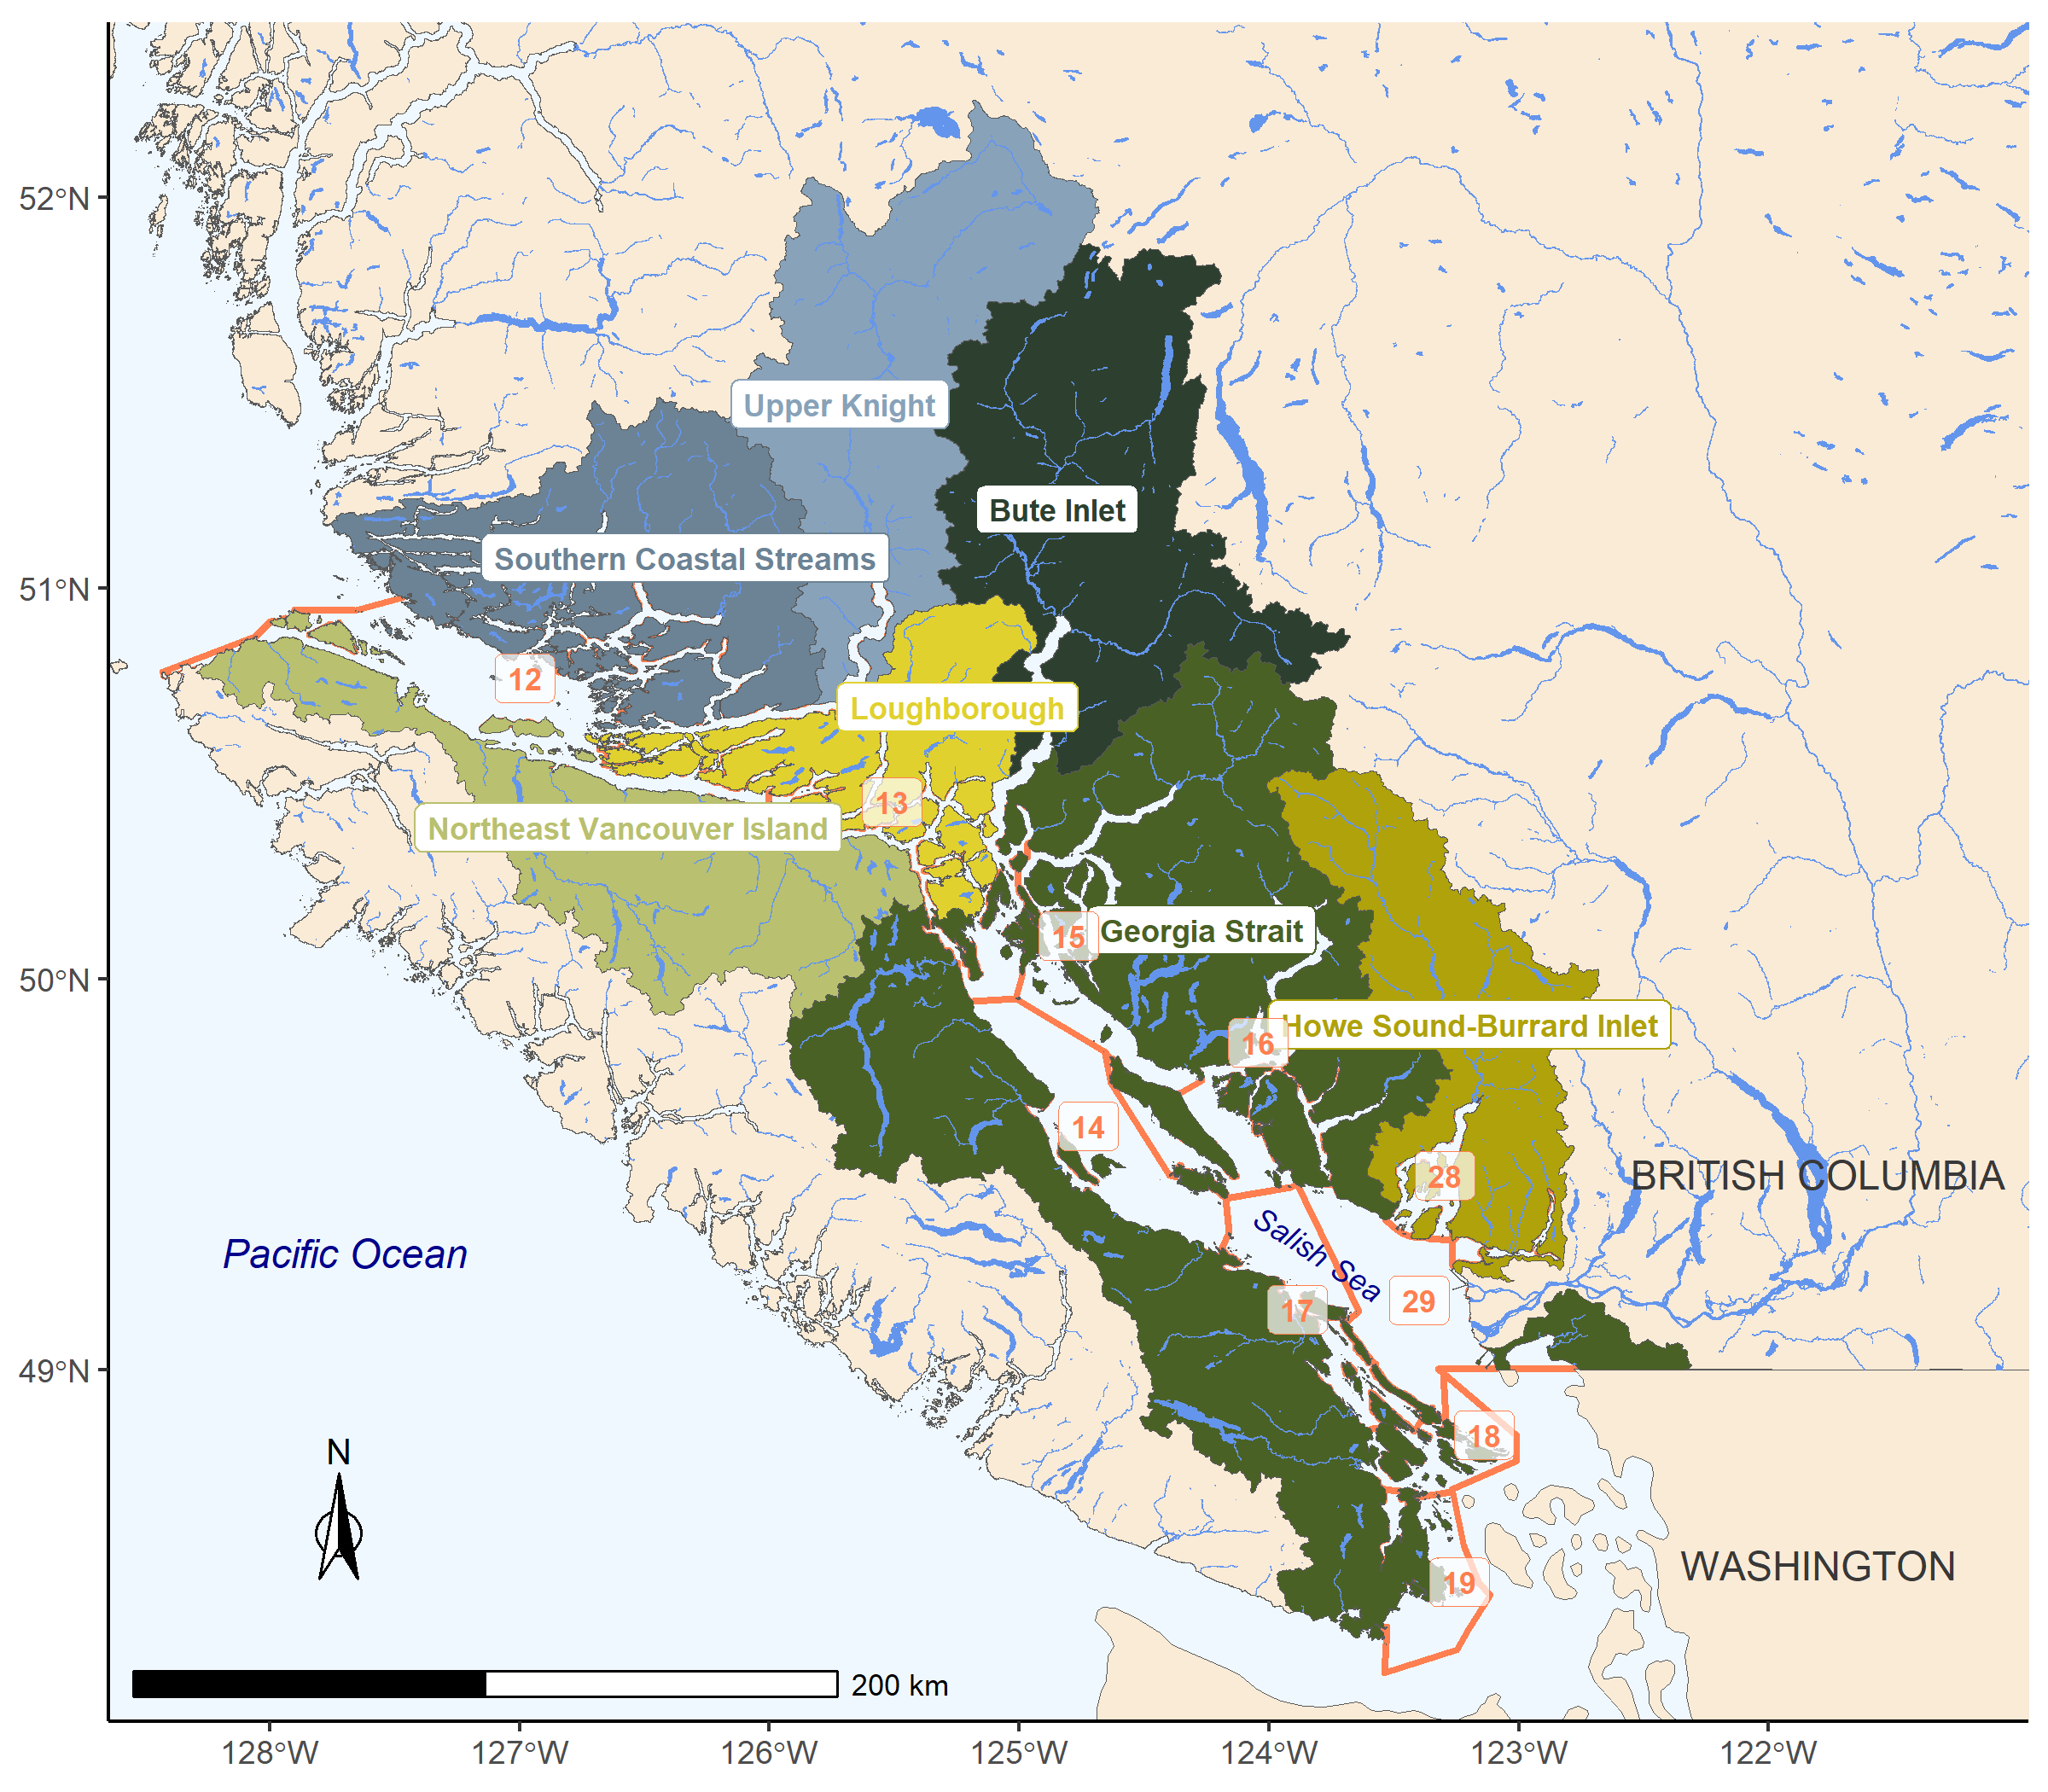
\includegraphics[width=6in]{C:/github/SalmonLRP_csasdown/caseStudyWP/figure/fig_chum_CU_map}}{Figure \ref{fig:chum-map}} 

}

\caption{The seven Conservation Units that make up the Inside South Coast Chum Stock Management unit (not including Lower Fraser and Fraser Canyon Conservation Units). Numbers indicate the Fishery Management Areas associated with these populations.}\label{fig:chum-map}
\end{figure}
\hypertarget{data-2}{%
\subsection{DATA}\label{data-2}}

We used essentially the same data used in \protect\hyperlink{ref-holt_evaluating_2018}{Holt et al.} (\protect\hyperlink{ref-holt_evaluating_2018}{2018}), updated with escapement data up to 2018. \protect\hyperlink{ref-van_will_inner_2014}{Van Will} (\protect\hyperlink{ref-van_will_inner_2014}{2014}) provides more details on the data sources, infilling procedures and run reconstruction, which were reproduced for this study and described below. We did not include the Lower Fraser or Fraser Canyon chum CUs.

\hypertarget{spawner-counts-escapement}{%
\subsubsection{Spawner counts / Escapement}\label{spawner-counts-escapement}}

We used spawning escapement data forom 1953-2018. Most of the escapement data comes from the NUSEDS database (a small amount from Lower Fraser Stock Assessment for Areas 28 and 29, FSC in-river catch from some First Nations, and enhanced escapement from DFO Salmon Enhancement Program) \emph{\textcolor{cyan}{LW: probably unneccesary detail}}. The number of chum salmon spawners that return to spawn (escapement) is typcially counted using visual surveys. Biologists from Fisheries and Oceans Canada and First Nations including \ldots{} (Island Marine Aquatic Working Group) \emph{\textcolor{cyan}{LW: which ones?}} generate these data by walking streams and counting fish, \emph{\textcolor{cyan}{LW: helicopter counts?}} and using fences or weirs on some rivers. Total escapement for each stream is usually a peak counts or estimated using the area under the curve (AUC) method.

\hypertarget{fishery-harvest-genetics-and-age}{%
\subsubsection{Fishery harvest, genetics, and age}\label{fishery-harvest-genetics-and-age}}

The number of chum caught in fisheries in the Inside South Coast area were taken from the DFO Clockwork Database, which includes the DFO Fishery Operating System and Sales slip databases and Genetic Stock Identification data. Age distributions for each year were taken from the Johnstone Strait fishery aggregate, as age data for specific CUs or streams was not available. Harvest data was not available for 1954-2018 \emph{\textcolor{cyan}{LW: confirm with Pieter Van Will why 1953 had no harvest data}}. Age composition data as available for 1958-2018.

\hypertarget{data-treatment}{%
\subsubsection{Data treatment}\label{data-treatment}}

We removed the summer run fish as all the data in regards the reconstruction work is associated with populations that return in the fall.

To get wild escapement, we kept only wild spawners, removing hatchery spawners, spawners harvested at a facility, and spawners collected for brood stock.

We also removed spawners for the Qualicum River, Little Qualicum River, and Puntledge River, as these systems have been nearly 100\% enhanced at least since enhancement began at these locations. We have little data in the enhanced contribution found in these returns but for the purposes of removing hatchery origin fish, we make the assumption that these streams had 100\% hatchery origin spawners.

After these removals, the steps for preparing the data for analysis were:
\begin{itemize}

\item
  Infill total and wild escapement by CU and Area, (by stream for CUs with observations, by CU for years with no observations in a CU)
\item
  Run reconstruction:
  \begin{itemize}

  \item
    Add fishery catch by CU and Area to total escapement to estimate total returns / recruitment / stock \emph{\textcolor{cyan}{LW: not sure which term to use here. Recruitment might be confusing since it is recruits in a spawning year, not for a brood year}}
  \item
    Use proportion of wild:total escapement by CU and Area to estimate number of wild returns
  \item
    Use age proportions of catch to estimate age of returns and get recruits by brood year for each CU. Result is wild spawners and corresponding recruits by brood year for each CU
  \end{itemize}
\end{itemize}
\hypertarget{infilling-of-spawner-escapement-data}{%
\subsubsection{Infilling of spawner escapement data}\label{infilling-of-spawner-escapement-data}}

The data we used had years where not all streams were counted. When a CU had some streams counted in a year, we infilled by stream (Figure~\ref{fig:chum-escapement-infill}). When there were no counts of spawners for a CU in a given year, we infilled by CU for that year and CU. We had to infill by CU to get total spawners to use for the run reconstruction, but we did not use CUs with CU-level infilling in the retrospective analysis of LRPs, as it assumes that escapement is correlated between CUs in a given year.

There were two puproses of infilling:
\begin{enumerate}
\def\labelenumi{\arabic{enumi}.}
\item
  Infill total and wild escapement by CU and Area in order to get wild returns by CU and Area, in order to estimate recruits for each brood year.
\item
  Infill wild escapement by CU, in order to get a time series of wild escapement to use in retrospective analysis of LRPs.
\end{enumerate}
\hypertarget{infilling-by-stream}{%
\paragraph{Infilling by stream}\label{infilling-by-stream}}

This applies to CUs and years when there were counts in some streams in the CU in a given year. For each stream, the geometric mean of escapement over all years was calculated as the stream's average escapement. Then the total average escapement for each CU in each year was the sum of the average escapements from all streams. Then a proportion of monitored escapement in each year was the sum of average escapement of all streams with counts in a year divided by the sum of the average escapements for all streams (counted and uncounted) in that CU. The infilled escapement for a CU in given year was the sum of the observed escapements for that CU and year divided by the proportion of the monitored escapement for that CU and year.

Infilling by stream typically made up a small proportion of the total escapement for each CU, with the exception of Howe Sound-Burrard Inlet. This was partly due to increasing escapements in the Cheakamus River and Indian River since 2000.

\hypertarget{infilling-by-cu}{%
\paragraph{Infilling by CU}\label{infilling-by-cu}}

If there were no counts of any streams in a CU in a given year, a second round of infilling was done with data set that had already been infilled by stream. This was the case for two CUs: Upper Knight (22 years: 1979-1980, 1982, 1984, 1989, 1991,1996,2004-18) and Bute Inlet (13 years: 2005-2006, 2008-2018).

Using by-stream infilled escapement summed for each CU, the CUs and years with missing data were infilled assuming the total CU escapement was correlated between CUs. The procedure was similar to that for infilling by stream, but a geometric average for each CU across all years was used to calculate the proportion of the average for each year, and then that was used to estimate escapement for the two CUs with no obervations.

\emph{\textcolor{cyan}{LW: This might be better in the discussion}} These CUs (Upper Knight and Bute Inlet) were not used for the retrospective analysis because the assumption that escapement is correlated between CUs ignores diversity between CUs and the potential for uncorrelated escapements. The reality of uncorrelated escapements must be taken into account to evaluate whether aggregate escapement is a meaningful predictor for the status of individual CUs. It should also be noted that these two CUs do not represent a random subset of the seven CUs in the Inside South Coast Chum SMU. Both have fewer streams than the other CUs and a higher proportion of summer-run populations of chum. These CUs also include long fjord systems with glaciers and watersheds that go deep into the mainland with headwaters in the Cariboo region. Environmental conditions including patterns of hydrology, geomorphology, and marine conditions when smolts enter the ocean in these systems may vary from that of the other five CUs, leading to differences in productivity and responses to the regional climate. For example, productivity (recruits per spawner) of the Upper Knight and Bute Inlet CUs (using CU-level infilling, which introduces error) have the largest magnitude of variability in the SMU, with very productive years (\textgreater100 recruits per spawner) and low productivity years, and boom and bust cycles of abundance. In other SMUs where the quality of data differs for a subset of CUs, careful consideration should be given to whether abundance, productivity, and their trends can be reliably estimated using data from CUs with data of higher quality.
\begin{figure}[htb]

{\centering \pdftooltip{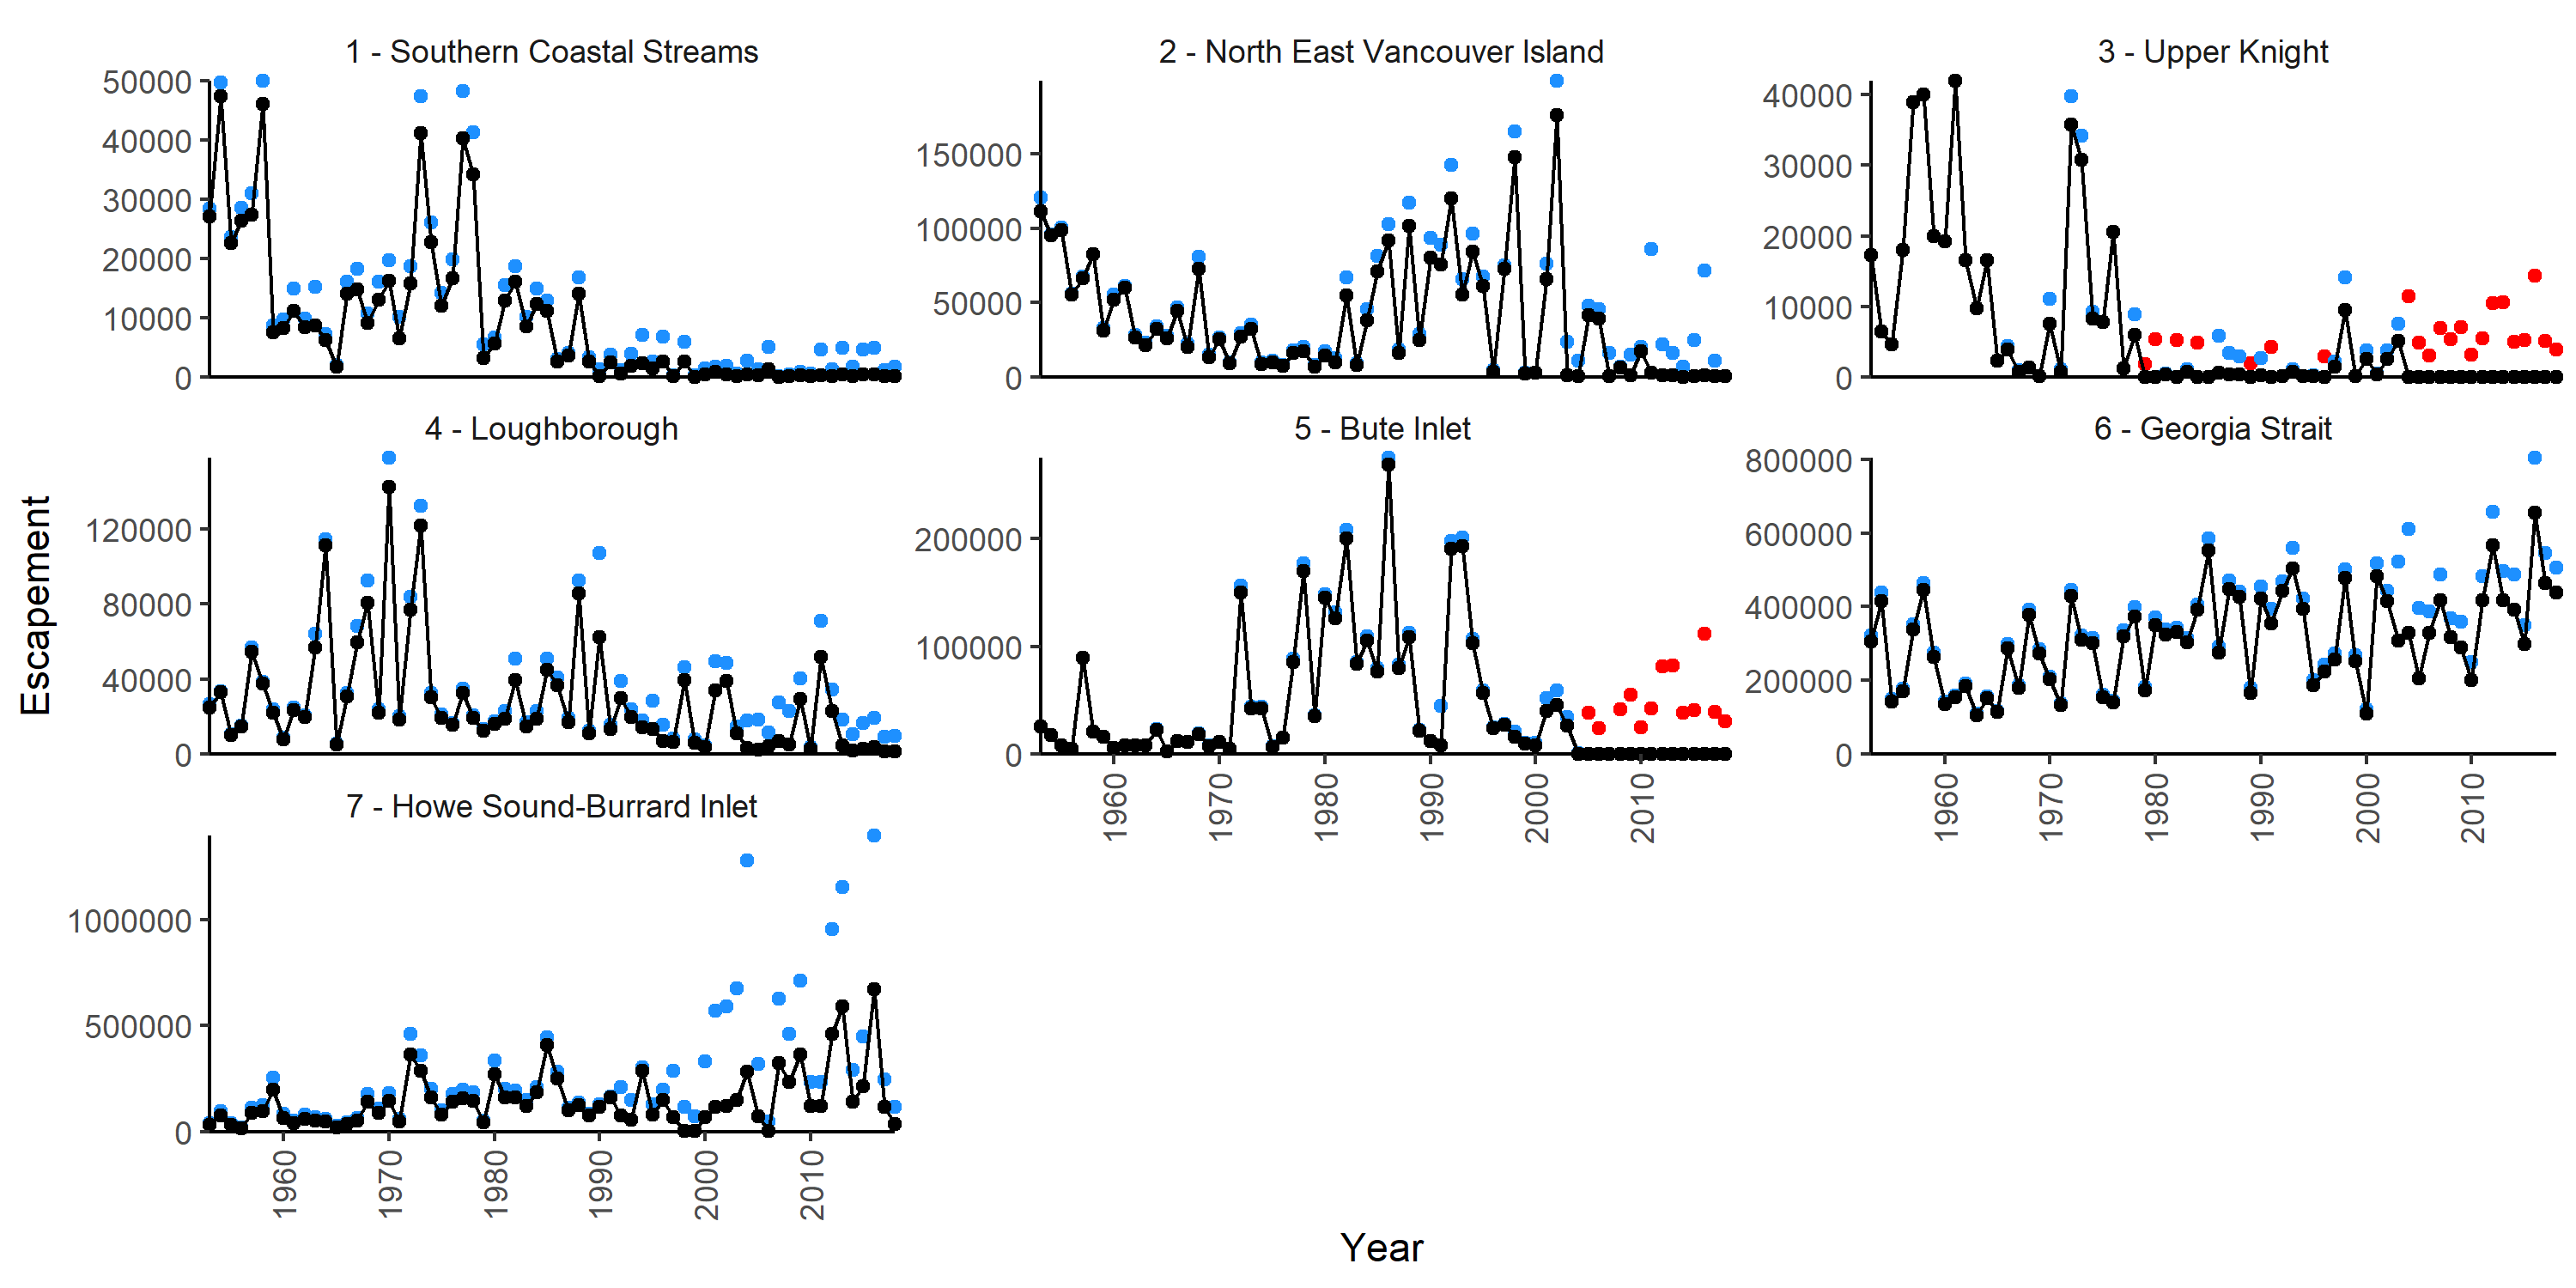
\includegraphics[width=6in]{C:/github/SalmonLRP_csasdown/caseStudyWP/figure/fig_compare_actual_infill_by_stream_and_CU}}{Figure \ref{fig:chum-escapement-infill}} 

}

\caption{Chum salmon escapement for the seven Conservation Units. Black points indicate actual counts, blue points are infilled by stream, and red points are infilled by Conservation Unit.}\label{fig:chum-escapement-infill}
\end{figure}
\hypertarget{run-reconstruction-to-estimate-recruitment}{%
\subsubsection{Run reconstruction to estimate recruitment}\label{run-reconstruction-to-estimate-recruitment}}

We reconstructed the returns for each brood year to give recruits for brood years 1955-2012 (age composition data from 1958-2018, minimum fish age was 3 years, maximum fish age was 6 years). Using CU benchmarks based on stock-recruit parameters - in this case, Sgen - requires knowing the spawners and recruits (adult offspring produced by each brood year of spawners) for each brood year (spawning year). Estimating recruits requires knowing wild spawner escapement, number of wild fish caught in fisheries, and the age of these fish.

To get these estimates, total (wild and hatchery origin) spawners based on the infilling methods above (both stream and CU level infilling) were calculated for each CU and Fishery Management Area (Figure~\ref{fig:chum-map}). The number of fish harvested in fisheries (wild and hatchery, by CU and Fishery Management Area) were added to the total escapement to get an estimate of totoal stock by CU and Fishery Management Area for each spawning year. This total stock number was multiplied by the proportion of wild spawners in each CU and Fishery Management Area based on the infilled wild and total spawner escapement. The product was an estimate of total wild stock (spawner escapement plus fishery harvest) by CU and Fishery Management Area for each brood year. Finally, the age composition of chum harvested in the Johnstone Strait aggregate fishery (ages 3, 4, 5 and 6) were used to assign fish from this total stock to brood years. As such, this analysis does not account for age diversity between CUs or streams.

Note that the two CUs requiring CU-level infilling correspond to only one Fishery Management Area each, which allows the run reconstruction using fishery harvest data at this level.

\hypertarget{methods-2}{%
\subsection{METHODS}\label{methods-2}}

\hypertarget{benchmarks-for-conservation-units}{%
\subsubsection{Benchmarks for Conservation Units}\label{benchmarks-for-conservation-units}}

\emph{\textcolor{cyan}{LW: some of this might be better in the lit review/ guidelines working paper}}
\begin{itemize}

\item
  The Wild Salmon Policy requires that salmon Conservation Units have set benchmarks dividing three levels of health: red, amber, green.
\item
  From \protect\hyperlink{ref-canada_canadas_2005}{\emph{Canada's policy for conservation of wild {Pacific} salmon}} (\protect\hyperlink{ref-canada_canadas_2005}{2005}): ``The lower benchmark between Amber and Red will be established at a level of abundance high enough to ensure there is a \textbf{substantial} buffer between it and any level of abundance that could lead to a CU being considered at risk of extinction by COSEWIC. The buffer will account for uncertainty in data and control of harvest management.''
\end{itemize}
Level of abundance that could lead to a CU being considered at risk of extinction by COSEWIC can be informed by several criteria:
\begin{itemize}

\item
  \protect\hyperlink{ref-holt_indicators_2009}{Holt et al.} (\protect\hyperlink{ref-holt_indicators_2009}{2009}): Table 2
  \begin{itemize}

  \item
    Spawner abundance
  \item
    Time trends in spawner abundance
  \item
    Distribution
  \item
    Likelihood of continued trends in abundance given fishing effort
  \end{itemize}
\item
  \protect\hyperlink{ref-cosewic_cosewic_2019}{COSEWIC} (\protect\hyperlink{ref-cosewic_cosewic_2019}{2019}): Table 2
  \begin{itemize}

  \item
    Decline in total number of mature individuals over last 10 years or 3 generations (whichever is longer) where reduction or its causes may not have ceased or may not be understood of may not be reversible, based on (and specifying) any of:
    \begin{itemize}

    \item
      direct observation
    \item
      an index of abundance appropriate to the taxon
    \item
      a decline in index of area of occupancy, extent of occurrence and/or quality of habitat
    \item
      actual or potential levels of exploitation
    \item
      the effects of introduced taxa, hybridization, pathogens, pollutants, competitors, or parasites
    \end{itemize}
  \item
    Reduction of \textgreater= 70\% = endangered
  \item
    reduction of \textgreater= 50\% = threatened
  \end{itemize}
\item
  \protect\hyperlink{ref-iucn_standards_and_petitions_committee_guidelines_2019}{Committee} (\protect\hyperlink{ref-iucn_standards_and_petitions_committee_guidelines_2019}{2019}): Table 2.1
  \begin{itemize}

  \item
    same as COSEWIC above, but uses ``Vulnerable'' instead of ``Threatened''
  \end{itemize}
\end{itemize}
How do these line up with LRPs?
\begin{itemize}

\item
  \protect\hyperlink{ref-government_of_canada_fishery_2009}{Government of Canada} (\protect\hyperlink{ref-government_of_canada_fishery_2009}{2009}): A fishery decision-making framework incorporating the precautionary approach:
  \begin{itemize}

  \item
    ``LRP represents the stock status below which serious harm is occurring to the stock.''
  \item
    ``At this stock level, there may also be resultant impacts to the ecosystem, associated species and a lont-term loss of fishing opportunities''
  \item
    ``When developing reference points efforts should be made to take into consideration the range of factors which may affect the productivity of the stock including changes in ocean conditions, where information is available.''
  \end{itemize}
\item
  \protect\hyperlink{ref-fisheries_and_oceans_canada_harvest_2006}{Canada} (\protect\hyperlink{ref-fisheries_and_oceans_canada_harvest_2006}{2006})
  \begin{itemize}

  \item
    ``The Limit reference point is the stock level below which productivity is sufficiently impaired to cause serious harm to the resource but \textbf{above the level where the risk of extinction becomes a concern}'' - Qualitatively similar to the benchmark between Red and Amber Zones in WSP.
  \end{itemize}
\end{itemize}
If each of the component CUs of a SMU is above the red/amber benchmark and thus not at risk of extinction, the entire SMU could judged to be above its LRP.

\hypertarget{appropriate-benchmarks-for-inside-south-coast-chum}{%
\subsubsection{Appropriate benchmarks for Inside South Coast Chum:}\label{appropriate-benchmarks-for-inside-south-coast-chum}}

Based on \protect\hyperlink{ref-government_of_canada_fishery_2009}{Government of Canada} (\protect\hyperlink{ref-government_of_canada_fishery_2009}{2009}): ``When developing reference points efforts should be made to take into consideration the range of factors which may affect the productivity of the stock including changes in ocean conditions, where information is available.''

Range of factors which may affect the productivity of Inside South Coast Chum:
\begin{itemize}

\item
  Ocean conditions:
  \begin{itemize}

  \item
    Competition / Biomass of North American pink, sockeye, and chum salmon \protect\hyperlink{ref-debertin_marine_2017}{Debertin et al.} (\protect\hyperlink{ref-debertin_marine_2017}{2017}), \protect\hyperlink{ref-litz_competition_2021}{Litz et al.} (\protect\hyperlink{ref-litz_competition_2021}{2021})
  \item
    Pacific Decadal Oscillation (PDO) (both positive and negative depending on what time period examined) \protect\hyperlink{ref-litz_competition_2021}{Litz et al.} (\protect\hyperlink{ref-litz_competition_2021}{2021})
  \item
    North Pacific Gyre Oscillation (NPGO) (positive relationship with growth), interaction between PDO and NPGO \protect\hyperlink{ref-debertin_marine_2017}{Debertin et al.} (\protect\hyperlink{ref-debertin_marine_2017}{2017})
  \item
    Early marine entry temperature (inlets)
  \item
    Timing of spring bloom
  \item
    Ocean ecology during time at sea (zooplankton, forage fish available) - dependent on ocean temperature \protect\hyperlink{ref-cheng_upper_2021}{Cheng et al.} (\protect\hyperlink{ref-cheng_upper_2021}{2021})
  \end{itemize}
\item
  Interacting / carry-over / complex effects:
  \begin{itemize}

  \item
    winter incubation temperatures -\textgreater{} earlier emergence -\textgreater{} potential mismatch with spring bloom Wilson 2021 thesis (chum outmigration getting earlier)
  \item
    ocean conditions -\textgreater{} female adult size -\textgreater{} egg burial depth * scour flood frequency/intensity (climate change) * land cover (exacerbating factors of floods) -\textgreater{} lower egg to adult survival
  \item
    female adult size -\textgreater{} egg size -\textgreater{} lower condition at estuary entry -\textgreater{} lower early marine survival
  \end{itemize}
\item
  Habitat loss
  \begin{itemize}

  \item
    estuary loss (human, climate change)
  \item
    change in quality of spawning habitat (change in sediment regime, possibly from forestry, landslides, potential climate change induced/exacerbated).
  \end{itemize}
\item
  Fishing mortality (Alaska, BC)
\item
  Predation
\end{itemize}
From \protect\hyperlink{ref-holt_evaluating_2018}{Holt et al.} (\protect\hyperlink{ref-holt_evaluating_2018}{2018}): ``Status assessments under the WSP integrate numerous metrics, including those on abundances, trends in abundance, and spatial distribution (Holt et al.~2009). Benchmarks on abundances (percentile or stock-recruitment based) are only one component of an integrated assessment of status that includes numerous other metrics (Grant and Pestal 2013; DFO 2015; DFO 2016).''

Based on the recommendations in \emph{Guidelines Working Paper}, we used benchmarks at the scale of Conservation Units to evaluate Limit Reference Points for Inside South Coast Chum. We compared two different benchmarks at the CU level: Sgen (based on Ricker parameters) and 25th percentile (based on historical abundance). these two benchmarks for Inside South Coast Chum. We used these benchmarks for this case study because of the previous work evaluating whether abundance-based benchmarks were appropriate for data-limited Chum populations (\protect\hyperlink{ref-holt_evaluating_2018}{Holt et al.} (\protect\hyperlink{ref-holt_evaluating_2018}{2018})).

Recommendations from \protect\hyperlink{ref-holt_evaluating_2018}{Holt et al.} (\protect\hyperlink{ref-holt_evaluating_2018}{2018}):

\hypertarget{benchmark-based-on-stock-recruit-relationship---sgen}{%
\subsubsection{Benchmark based on stock-recruit relationship - Sgen}\label{benchmark-based-on-stock-recruit-relationship---sgen}}

For Inside South Coast chum, there are no reliable data on marine survival for wild fish, and no proxies based on coded wire tag or age at return of hatchery chum in this SMU. This meant that the Ricker model used to estimate the spawner-recruit relationship did account for marine survival (compared to Interior Fraser Coho).

We used a basic Ricker model to estimate the the predicted recruits \(\hat{R}\) from spawners \(S\), productivity \(\alpha\), and the strength of density dependence \(\beta\) for each stock \(i\)~\ref{eq:ricker}. We used the log-transformed Ricker equation so that the residuals/error would be normally distributed~\ref{eq:log-ricker}. \emph{\textcolor{cyan}{LW: is this correct about the residuals/error?}}
\begin{equation}
    log(R) = \alpha \centerdot S e^{-\beta * S} 
    \label{eq:ricker}
\end{equation}
\begin{equation}
  log(\hat{R}) = log(\alpha_i) + log(S) - e^{log(\beta_i)} * S 
  \label{eq:log-ricker}
\end{equation}
Warnings with Sgen / ricker based benchmarks:
\begin{itemize}

\item
  Ignores variability in actual recruits/spawner (Sgen is based on mean \alpha value). This can be problematic if there are large residuals (especially negative) in the stock-recruit curve at low spawner abundance. For example, if 20\% of the time (based on record of recruits/spawner), Sgen spawners actually had recruits/spawner less than 1. Then you set up a potential tail-spin to low abundance, depending on the frequency of these low recruitment cohorts at low abundance.
\item
  Because they are set at the CU level (high level in terms of stock-recruit relationship, not at the scale of stream-level density-dependence or ocean-level density dependence including overlapping species (e.g., Alaska, pacific ocean)), they may not explicitly model density dependence at scales where it is probably occurring.
\item
  Assumes productivity and density-dependence are constant (not true, especially given the importance of biomass of pinks for chum salmon, ocean food availability)
\item
  \alpha and \beta are negatively correlated: sensitive to each other, especially when fit is not good, this is problematic, especially since \(S_MSY\) and \(S_gen\) depend on both \alpha and \beta
\item
  \(MSY\) and its derivatives (e.g., \(S_MSY\), \(S_gen\)) are not based on COSEWIC risk of extinction metrics such as percent decreases in spawner abundance
\end{itemize}
\hypertarget{benchmark-based-on-historical-abundance---percentile}{%
\subsubsection{Benchmark based on historical abundance - Percentile}\label{benchmark-based-on-historical-abundance---percentile}}

\protect\hyperlink{ref-hilborn_british_2012}{Hilborn et al.} (\protect\hyperlink{ref-hilborn_british_2012}{2012}) used a percentile approach for Interior South Coast chum salmon

Warnings with percentile approach:
\begin{itemize}

\item
  Shifting baselines
\item
  Assumes productivity (recruits/spawner) stationary
\item
  record only starts with data
\item
  Accounting for fishing mortality? percentile of recruits vs.~escapement
\end{itemize}
\hypertarget{other-considerations-of-benchmarks}{%
\subsubsection{Other considerations of benchmarks}\label{other-considerations-of-benchmarks}}
\begin{itemize}

\item
  \% decreases in abundance
\item
  Time frame (10 years / 3 generations)
\item
  Consideration of causes and a higher level of caution: ``where reduction or its causes may not have ceased or may not be understood of may not be reversible''
\end{itemize}
\hypertarget{regression-forms}{%
\subsubsection{Regression forms}\label{regression-forms}}

Bernoulli vs.~Binomial Regression forms are described in \protect\hyperlink{logistic-regression-lrps}{Chapter 2}

\hypertarget{empirical-lrps-2}{%
\subsubsection{EMPIRICAL LRPS}\label{empirical-lrps-2}}
\begin{itemize}
\item
  We evaluate two empirical (data-based) approaches for developing aggregate abundance-based LRPs for Inside South Coast Chum using the 5 CUs with \textgreater{} 15 years of data {[}not sure this is the best way to descibe??; please fix{]}. Both approaches attempted to estimate LRPs by fitting logistic regression models to historically observed data; they differ in the metric used to represent CU-level lower benchmarks.
\item
  The first approach uses Sgen \ldots{}
\item
  The second approach used percentile-based benchmarks \ldots{}
\item
  Due to poor logistic model fits using the entire 19xx - 2018 time series for both Sgen and percentile benchmarks, we did not conduct retrospective analyses for this SMU. The underlying data characteristics that lead to poor logsitic model fits are highlighted in the results section below.
\end{itemize}
\hypertarget{projected-lrps-tbd}{%
\subsubsection{PROJECTED LRPS (TBD)}\label{projected-lrps-tbd}}

\hypertarget{multidimensional-approach-tbd}{%
\subsubsection{MULTIDIMENSIONAL APPROACH (TBD)}\label{multidimensional-approach-tbd}}

Data and methods are available at: \url{https://github.com/Pacific-salmon-assess/SalmonLRP_RetroEval}.

\hypertarget{results-2}{%
\subsection{RESULTS}\label{results-2}}

\hypertarget{empirical-lrps-3}{%
\subsubsection{EMPIRICAL LRPS}\label{empirical-lrps-3}}
\begin{itemize}

\item
  Show poor model fits for each benchmark (using Bernoulli)
\item
  Summarize model fit diagnostics
\item
  Highlight low covariance and differences in scale, and describe how these make empirical LRPs unsuitable for this SMU
\item
  Also - include plots showing variation in Sgen and percentile benchmarks over time for the 5 CUs to highlight time-varying concerns.
\end{itemize}
\hypertarget{projected-lrps-tbd-1}{%
\subsubsection{PROJECTED LRPS (TBD)}\label{projected-lrps-tbd-1}}

\hypertarget{multidimensional-approach-tbd-1}{%
\subsubsection{MULTIDIMENSIONAL APPROACH (TBD)}\label{multidimensional-approach-tbd-1}}

\hypertarget{lessons-learned-from-case-study-applications}{%
\section{LESSONS LEARNED FROM CASE STUDY APPLICATIONS}\label{lessons-learned-from-case-study-applications}}
\begin{itemize}

\item
  SYnthesize main results and conclusions from case studies
\end{itemize}
\clearpage

\hypertarget{references}{%
\section{REFERENCES}\label{references}}

% This manually sets the header for this unnumbered chapter.
\noindent
\vspace{-2em}
\setlength{\parindent}{-0.2in}
\setlength{\leftskip}{0.2in}
\setlength{\parskip}{8pt}

\hypertarget{refs}{}
\begin{CSLReferences}{1}{0}
\leavevmode\hypertarget{ref-fisheries_and_oceans_canada_harvest_2006}{}%
Canada, F. and O. 2006. A harvest strategy compliant with the precautionary approach. Fisheries; Oceans Canada.

\leavevmode\hypertarget{ref-canada_canadas_2005}{}%
Canada's policy for conservation of wild {Pacific} salmon. 2005. Fisheries; Oceans Canada, Vancouver.

\leavevmode\hypertarget{ref-cheng_upper_2021}{}%
Cheng, L., Abraham, J., Trenberth, K.E., Fasullo, J., Boyer, T., Locarnini, R., Zhang, B., Yu, F., Wan, L., Chen, X., Song, X., Liu, Y., Mann, M.E., Reseghetti, F., Simoncelli, S., Gouretski, V., Chen, G., Mishonov, A., Reagan, J., and Zhu, J. 2021. Upper {Ocean} {Temperatures} {Hit} {Record} {High} in 2020. Advances in Atmospheric Sciences 38(4): 523--530.

\leavevmode\hypertarget{ref-iucn_standards_and_petitions_committee_guidelines_2019}{}%
Committee, I.S. and P. 2019. Guidelines for {Using} the {IUCN} {Red} {List} {Categories} and {Criteria}. Prepared by the Standards; Petitions Committee.

\leavevmode\hypertarget{ref-cosewic_cosewic_2019}{}%
COSEWIC. 2019. {COSEWIC} {Assessment} {Process}, {Categories} and {Guidelines}.

\leavevmode\hypertarget{ref-debertin_marine_2017}{}%
Debertin, A.J., Irvine, J.R., Holt, C.A., Oka, G., and Trudel, M. 2017. Marine growth patterns of southern {British} {Columbia} chum salmon explained by interactions between density-dependent competition and changing climate. Canadian Journal of Fisheries and Aquatic Sciences 74(7): 1077--1087.

\leavevmode\hypertarget{ref-government_of_canada_fishery_2009}{}%
Government of Canada, F. and O.C. 2009, March. A fishery decision-making framework incorporating the precautionary approach.

\leavevmode\hypertarget{ref-hilborn_british_2012}{}%
Hilborn, R., Schmidt, D., English, K., and Devitt, S. 2012. British {Columbia} {Chum} {Salmon} (\emph{{Oncorhynchus} keta}) {Fisheries}: {British} {Columbia} {Coastal} and {Adjacent} {Canadian} {Pacific} {EEZ} {Waters}, {Final} {Certification} {Report}. Submitted to Canadian Pacific Sustainable Fisheries Society.

\leavevmode\hypertarget{ref-holt_indicators_2009}{}%
Holt, C.A., Cass, A., Holtby, B., and Riddell, B. 2009. Indicators of {Status} and {Benchmarks} for {Conservation} {Units} in {Canada}'s {Wild} {Salmon} {Policy}.~: 82.

\leavevmode\hypertarget{ref-holt_evaluating_2018}{}%
Holt, C., Davis, B., Dobson, D., Godbout, L., Luedke, W., and Tadey, J. 2018. Evaluating {Benchmarks} of {Biological} {Status} for {Data}-limited {Conservation} {Units} of {Pacific} {Salmon}, {Focusing} on {Chum} {Salmon} in {Southern} {BC}.~: 87.

\leavevmode\hypertarget{ref-holtby_conservation_2007}{}%
Holtby, L.B., and Ciruna, K.A. 2007. Conservation {Units} for {Pacific} {Salmon} under the {Wild} {Salmon} {Policy}. Research \{Document\}, Fisheries; Oceans Canada.

\leavevmode\hypertarget{ref-litz_competition_2021}{}%
Litz, M., Agha, M., Dufault, A., Claiborne, A., Losee, J., and Anderson, A. 2021. Competition with odd-year pink salmon in the ocean affects natural populations of chum salmon from {Washington}. Marine Ecology Progress Series 663: 179--195.

\leavevmode\hypertarget{ref-van_will_inner_2014}{}%
Van Will, P. 2014. Inner {South} {Coast} {Chum} {Stock} {Reconstructions} (1953-2013).

\end{CSLReferences}
\setlength{\parindent}{0in} \setlength{\leftskip}{0in} \setlength{\parskip}{4pt}

\Appendices


\clearpage

\refstepcounter{chapter}
\label{app:first-appendix}
\starredchapter{APPENDIX~\thechapter. THE FIRST APPENDIX}

Content here.


\clearpage

\refstepcounter{chapter}
\label{app:second-appendix}
\starredchapter{APPENDIX~\thechapter. THE SECOND APPENDIX, FOR FUN}

More content.

\end{document}
